\documentclass[a4paper]{extarticle}
\usepackage[utf8]{inputenc}
\usepackage[a4paper, margin=1in]{geometry}

\usepackage{amssymb}
\usepackage{amsmath}
\usepackage{enumitem}
\usepackage{tcolorbox}
\usepackage{fancyhdr}
\usepackage{graphicx}
\usepackage{float}

\setlength{\parindent}{0em}
\setlength{\parskip}{0.4em}

\definecolor{theoremblue}{RGB}{1, 73, 124}
\definecolor{corollaryblue}{RGB}{70, 143, 175}
\definecolor{exampleblue}{RGB}{137, 194, 217}

\newtcolorbox{tbox}{colback=theoremblue!20,colframe=theoremblue,
boxrule=0pt,arc=0pt,boxsep=2pt,left=2pt,right=2pt,leftrule=2pt}

\newtcolorbox{cbox}{colback=corollaryblue!20,colframe=corollaryblue,
boxrule=0pt,arc=0pt,boxsep=2pt,left=2pt,right=2pt,leftrule=2pt}

\newtcolorbox{ebox}{colback=exampleblue!20,colframe=exampleblue,
boxrule=0pt,arc=0pt,boxsep=2pt,left=2pt,right=2pt,leftrule=2pt}

\title{EnpRisk - Lecture Notes Week 13}
\author{Ruben Schenk, ruben.schenk@inf.ethz.ch}
\date{\today}

\pagestyle{fancy}
\fancyhf{}
\rhead{ruben.schenk@inf.ethz.ch}
\rfoot{Page \thepage}
\lhead{EnpRisk - Lecture Notes Week 13}

\begin{document}

\maketitle

\section{How to Prepare for the Great Shifts}

\subsection{The Secret History of Silicon Valley}

Short overview of the Silicon Valley:

\begin{itemize}
    \item Terman/Stanford/Government is responsible for entrpreneurial culture of Silicon Valley
    \item Military primed the pump as a customer for key Valley technologies (Semiconductors, computers, the Internet etc.)
    \item Venture Capital turned the Valley to volume corporate and consumer applications
    \item Berkeley continued its focus on Big Science and National Labs
\end{itemize}

\begin{figure}[H]
    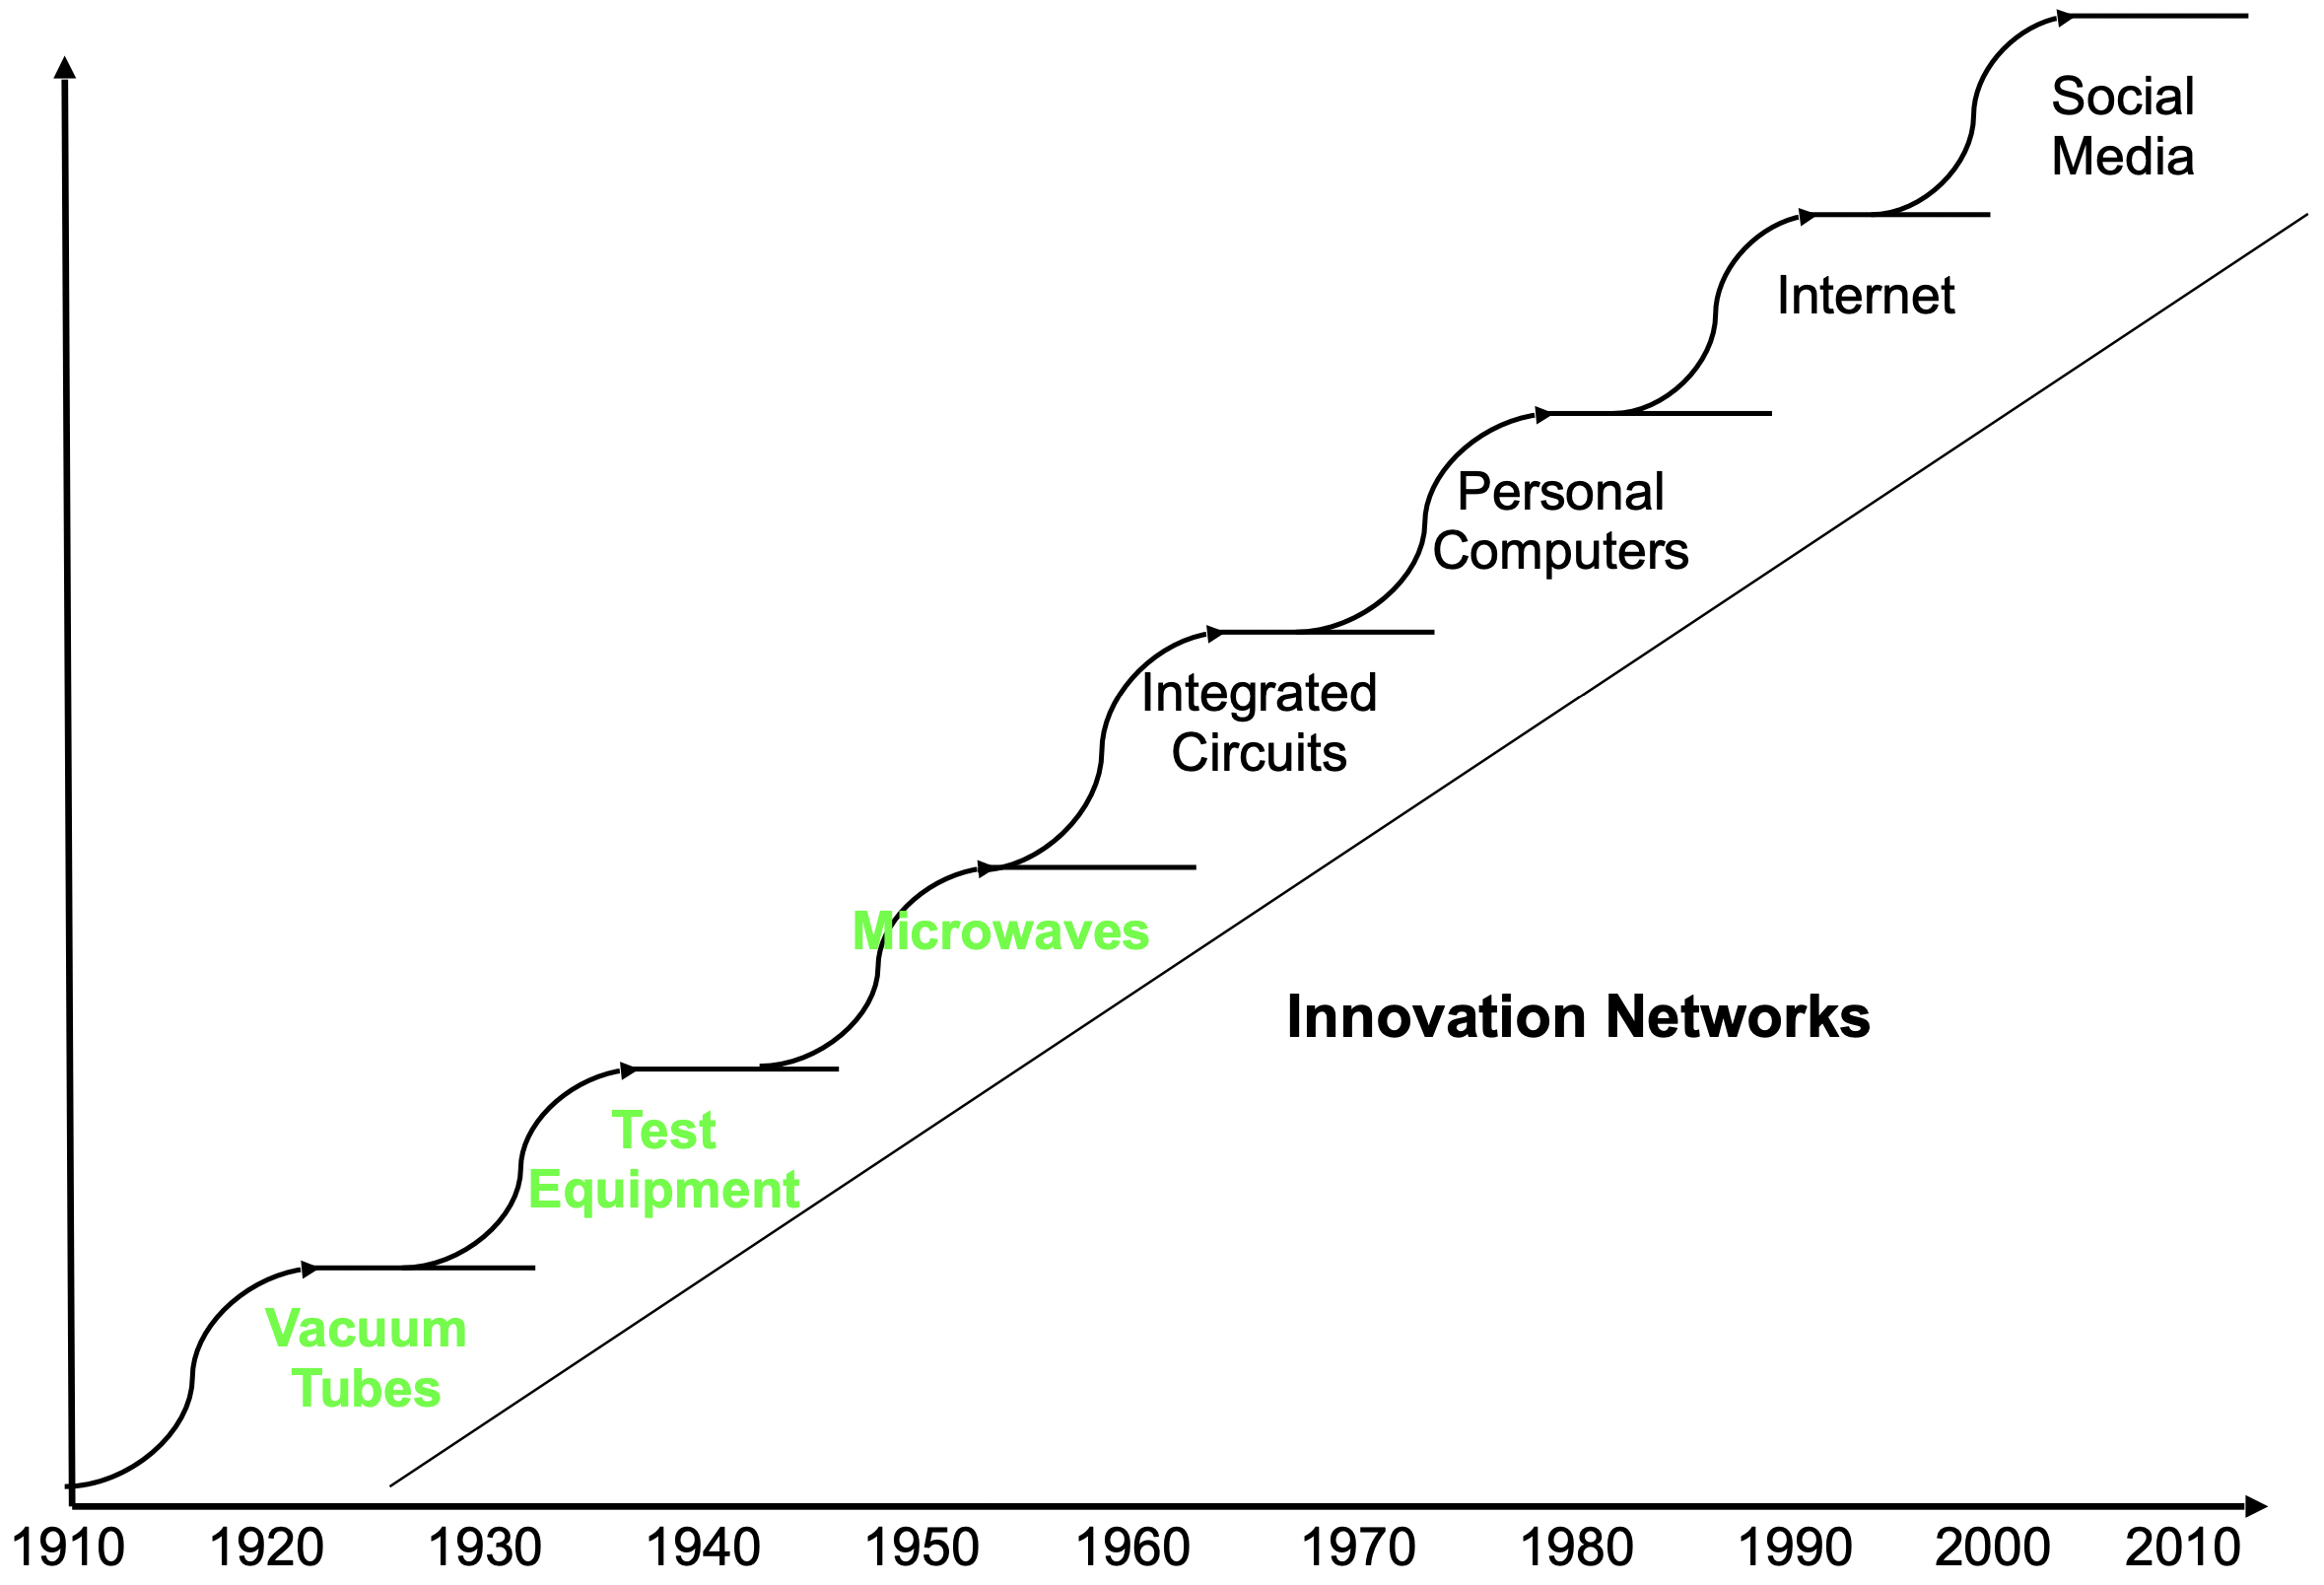
\includegraphics[width=15cm]{../images/EnpRisk_Fig13-1}
    \centering
\end{figure}

In particulare, the time of "Microwaves" also included \textbf{defenese!}

For example, during WWII one encountered the first electronic war. Germany created the first air defense systems, i.e. integrated electronic air defense networks which covered France, the Low Countries, and into northern Germany. By AQugust 1941, only $10\%$ of British bombers got to within 10 miles of their target.

In response, the Harvard Radio Research Lab (RRL) was created which focused on signals intelligence and electronic warfare:

\begin{itemize}
    \item Reduce losses to fighters and flak
    \item Find and understand German air defense
    \item Jam and confuse German air defense
    \item Top secrete 800-person lab
\end{itemize}

The Harvard RRL was separate from MIT's Radiation Laboratory and ran all electronic warfare in WWII. It consisted of 800 people and was active from 1941 until 1944. The director was \textit{Frederick Terman} from the Stanford University, a Stanford Professor of engineering 1926.

Terman's post-war strategy was as follows:

\begin{itemize}
    \item Focus on microwaves and electronics (not going to be left out ov governemtns \$ this time)
    \item Recruit 11 former members of RRL as faculty
    \item Set up the Electronics Research Laboratory (ERL)
    \item First Office of Naval Research (ONR) contract in 1946
    \item By 1950, Stanford was the MIT of the West
\end{itemize}

The Cold War battlefield moves 500 miles east. Countermeasures become critical and Stanford becomes the center of excellence for the CIA, NSA, Navy, and the Air Force. Stanford house a 400-person weapons lab in the engineering department.

After all of that, Terman changed the startup/University rules:

\begin{itemize}
    \item Graduate students were encourages to start companies
    \item Professors were encouraged to consult for these companies
    \item Terman and other professors took board seats
    \item Technology transfer and IP licensing was made easy
    \item Getting out into the real world was good for your academic career
    \item Failure was accepted as part of the culture
\end{itemize}

Terman's strategy was a follows:

\begin{enumerate}
    \item Sit on every possible Military Advisory board (build network and relationships)
    \item Reach out to military customers to understand their needs. Then craft a prototype in Stanford's labs (generate revenue for the university and strengthen its military relationship)
    \item If the customer liked the prototype, encourage a student to found a company and manufacture at scale (inspired entrepreneurship and hard work in the students in the university's labs)
    \item Put a Stanford faculty (or Terman) on the board or as a consultant with the new company (train Stanford faculty in business and turn them into better teachers and researchers)
    \item Provide office space in the Stanford Industrial Park (ensure that the startup stays close and helps the entrepreneurial ecosystem reach a higher density)
\end{enumerate}

The \textit{Other Father of Sillicon Valley} was William Shockley. He was the Co-inventor of the transistor for which he won a Nobel Prize in 1956 anf founded Shockley Transistor 1955, the first semiconductor company in California.

Silicon Valley's 2nd engine of entrepreneurship was \textit{venture capital.} Raise money from pension funds, private universities, and wealthy individuals - the limited partners. Investment professionals manage the fund - the general partners, i.e. the VC's.

\begin{figure}[H]
    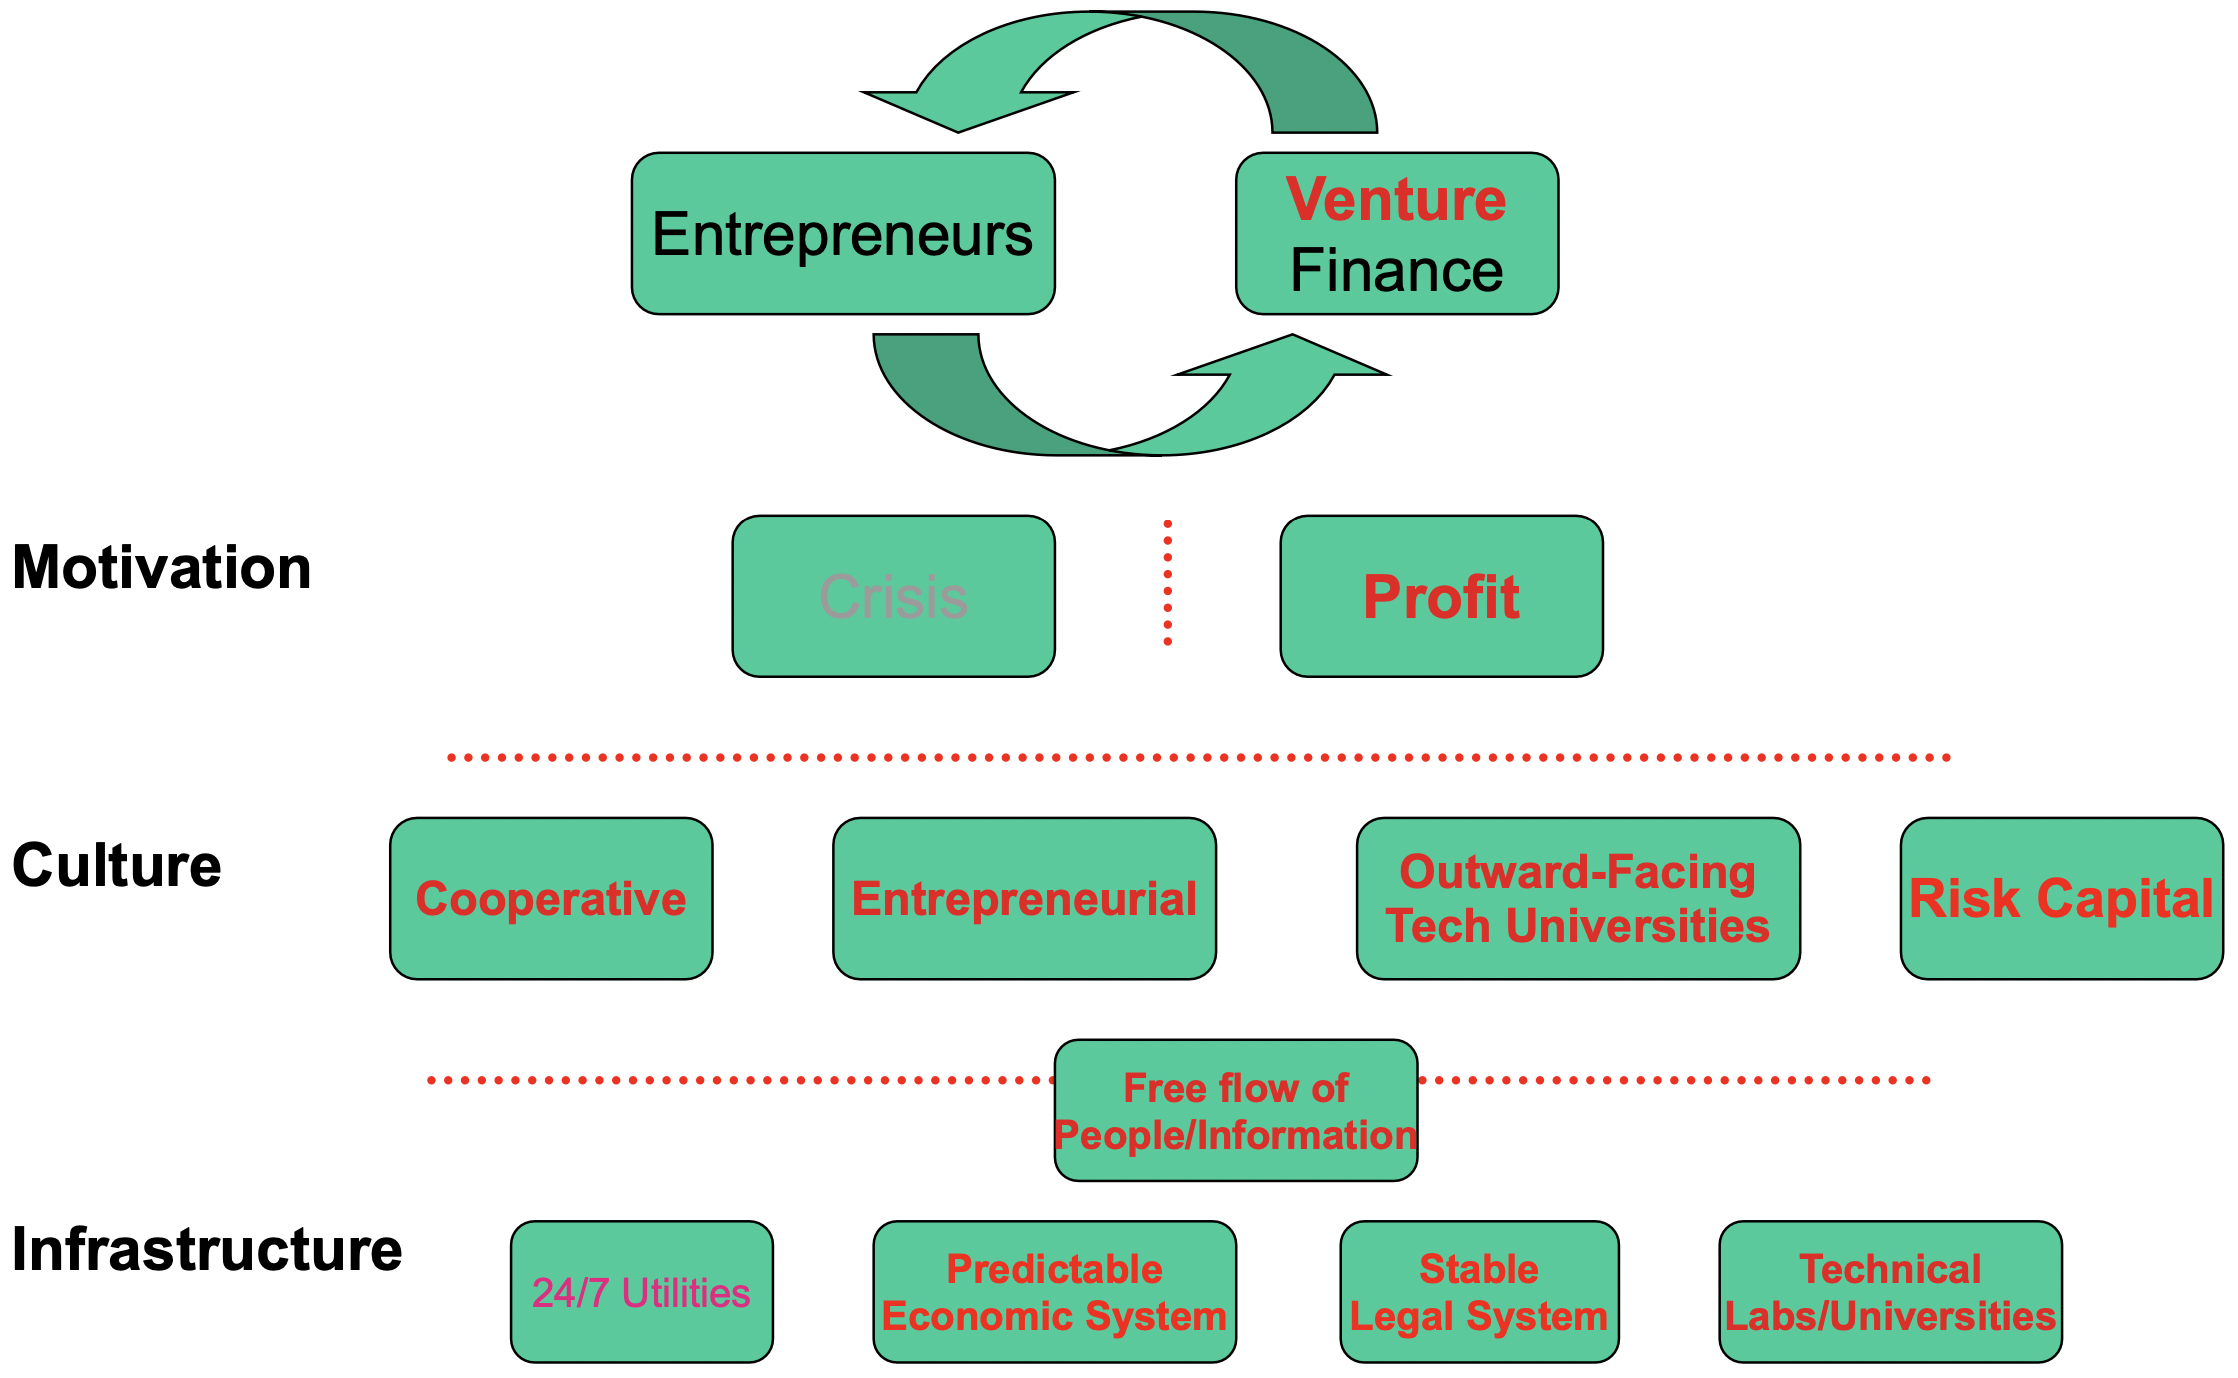
\includegraphics[width=15cm]{../images/EnpRisk_Fig13-2}
    \centering
\end{figure}

Venture capital turned the Valley to volume corporate and consumer applications.

\subsection{The Social Bubble Hypothesis}

A \textbf{social bubble} developing during a technological project is defined when several of the following symptoms are simultaneously present:

\begin{itemize}
    \item strong growth of presence in the media, newspapers, books, blogs, grossips, cocktails, etc.
    \item flow of venture capital and Wall Street investments
    \item accelerated price growth of corresponding firms trading on organized stock markets
    \item proliferation of ventures of all kinds
\end{itemize}

\subsubsection{Example: The Human Genome Project}

In February 2001, Celera and HGP scientists published details of their drafts, describing the methods used and offering analysis of the sequence. However, anticipations of the commercial and medical applications of the HGP were highly inflated.

Today, it is acknowledge that insight into the genetic mapping and sequencing effort is only seen as a starting point for future research in biology and medicin. Contrary to claims during its development, the main fruits of the HGP have been accuring to the research community, and almost nothing to medicine and the general public.

Still, indirect technological gains values at $> 750$ Billion USD by Obama's administration.

From 2004 to 2008, a bubble formed in \textit{clean technologies,} such as solar, biofuels, batteries, and other renewable energy sources. This \textbf{clean-tech bubble} can be rationalised through the lens of the interactions between enthusiastic supporters weave a network of reinforcing feedbacks that lead to widespread endorsement and extraordinary commitment by those involved.

The clean-tech bubble was clearly a social bubble: the narrative of a "moral imperative" to combat climate change and achieve "salvation", the ballooning venture capital investments, and the massive government subisides weaved a network of self-reinforcing spirals that lead to over-optimsitic expectations, excessive enthusiasm, and over-investments.

Although the clean-tech bubble bust, we can identify some factors that indicate that the bubble did indeed catalyze technological progress in clean and renewable energy technologies.

\subsection{John Boyd's Strategy in the 21st Century}

The OODA (Observe, Orient, Decide and Act) loop with power:

\begin{figure}[H]
    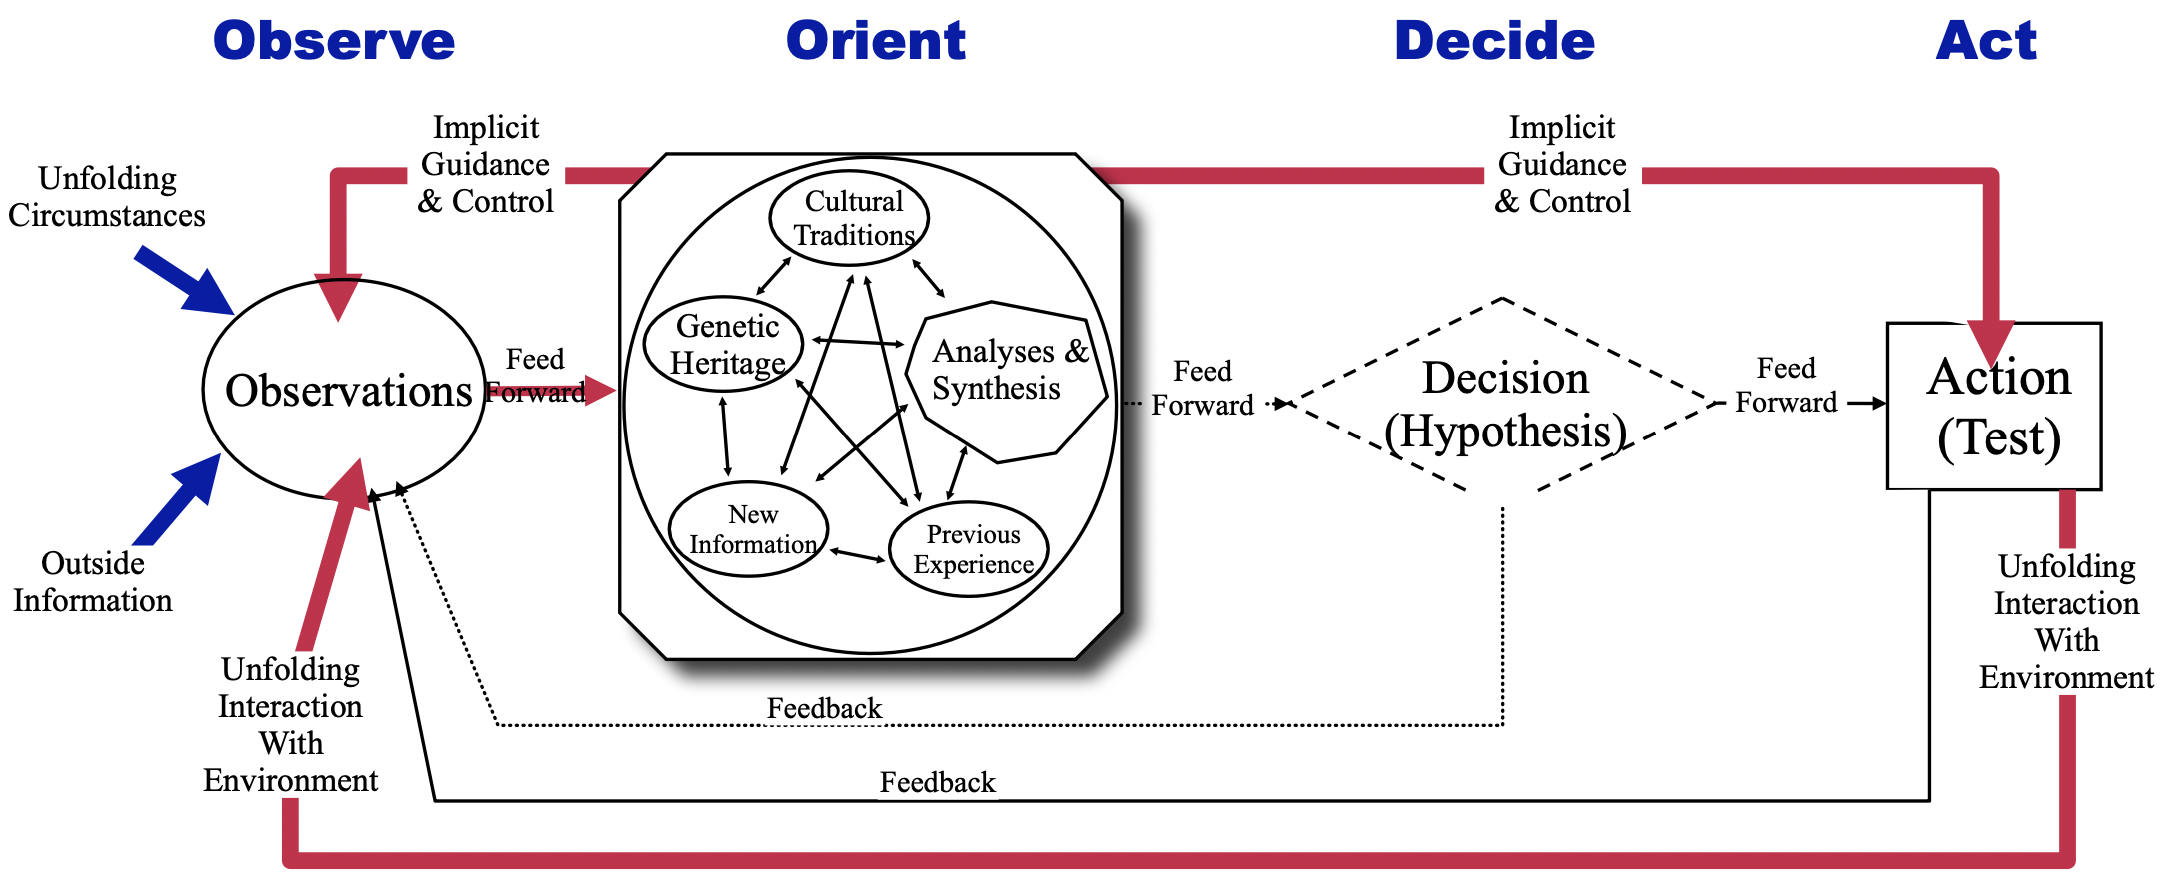
\includegraphics[width=15cm]{../images/EnpRisk_Fig13-3}
    \centering
\end{figure}

The key take-aways is that \textit{time is special.} Time is the only physical parameter with a direction. You don't have an unlimited supply, once it's gone, it's gone. Sure sign you're not using Boyd's strategies: you try to solve problems by throwing more time at them. A time-compressed company does the same thing as a pilot in an OODA loop. It's the competitor who acts on information faster who is in the best position to win.

\subsubsection{Boyd's organizational climate}

The principles of the Blitzkrieg:

\paragraph{Fingerspitzengefühl} Zen-like quality of intuitive understanding. Ability to sense when the time is ripe for action. Built through years of progressively more challenging experience.

\paragraph{Einheit} Has the connotation of "mutual trust" and implies a common outlook towards business problems. Built through common experience. Fingerspitzengefühl at the organizational level.

\paragraph{Schwerpunkt} Any concept that gives focus and direction to our efforts. In ambiguous situations, answer the question, "What do I do next?". Requires leadership.

\paragraph{Auftragstaktik} Tell team members what needs to be accomplished, get their agreement to accomplish it, then hold them strictly accountable for doing it - but don't prescribe how. Requires very high levels of mutual trust.

\end{document}